\chapter{The Solow Growth Model}

The Solow model is the fundamental workhorse of economic growth theory, focusing on how \textbf{capital accumulation} drives output growth over time. Its economic intuition rests on two core properties of physical capital:
\begin{itemize}
    \item \textbf{Rivalry and Diminishing Returns:} Capital is a rival good. As we equip a fixed number of workers with more and more machines, the marginal contribution of each additional machine declines.\footnote{
        To build intuition for why rivalry causes diminishing returns, consider the ``congestion" of physical tools. If a single worker is given one unit of capital (e.g., a machine), there is no conflict. If a second unit is added, the two machines must now compete (or ``conflict") for the same worker's fixed physical attention. This congestion dictates that the second machine cannot contribute as much as the first. A third machine creates even more conflict, yielding an even smaller marginal gain. 

In contrast, a non-rival factor (like a software algorithm, a blueprint, or a scientific formula) does not suffer from this physical congestion. A single idea can be applied to all machines and workers simultaneously without being depleted. Therefore, an improvement in a non-rival factor acts as a direct multiplier to overall output, avoiding the trap of diminishing marginal returns.
    }
    \item \textbf{Durability and Depreciation:} Capital is durable, allowing it to be accumulated over time, which generates a dynamic growth path. However, it also depreciates, meaning continuous investment is required to maintain the stock.
\end{itemize}

\noindent Key Takeaways from the Solow Model:
\begin{itemize}
    \item \textbf{Long-Run Stagnation:} Due to diminishing returns to capital, growth driven solely by capital accumulation will eventually slow down and cease.
    \item \textbf{Transitional Dynamics:} Economies that start with a low initial capital stock will experience strong ``catch-up growth" as they converge to their steady state.
\end{itemize}

\section{The Economic Environment}

\begin{itemize}
    \item \textbf{Time:} Discrete time, $t = 0,1,2,\cdots$.
    \item \textbf{Production Function:} In each period, the total output $Y_t$ is produced using physical capital $K_t$ and labor $L$:
    $$
    Y_t = A F(K_t,L)
    $$
    where the technology level $A$ is exogenously given and fixed. 
    \rmkb[]{
        In reality, output depends on total \textit{effective labor} (namely the human capital, $H$), which incorporates workers' education and skills (i.e., $H = h \cdot L$, where $h$ is human capital per worker). However, in the baseline Solow model, we deliberately make two independent simplifying assumptions to isolate the mechanics of physical capital ($K$):
    \begin{enumerate}
        \item We abstract away from skill accumulation by assuming all workers are identical and have a constant baseline skill level ($h=1$). Thus, human capital reduces to raw headcount: $H = L$.
        \item We abstract away from population dynamics by assuming the raw labor force $L$ is fixed and given (i.e., population growth rate $n=0$).
    \end{enumerate}
    By shutting down the channels from both the education and the population, we force physical capital accumulation to be the sole driver of transitional growth in this baseline model.
    }
    \item \textbf{Diminishing Returns to Capital:} The production function $F(\cdot)$ is strictly concave in capital, meaning that the marginal product of capital decreases as we accumulate more capital. Formally, we assume $F_K > 0$ and $F_{KK} < 0$.
    
    In addition, we assume the production function $F(\cdot)$ exhibits \textit{Constant Returns to Scale (CRS)}. This allows us to divide both sides by $L$:
$$
y_t = A F\left(\frac{K_t}{L}, 1\right) \equiv A f(k_t)
$$
where $f'(k_t) > 0$ and $f''(k_t) < 0$, capturing the strictly positive but diminishing marginal product of capital. 
    \item \textbf{Law of Motion for Capital}: The evolution of the aggregate capital stock is governed by:
$$
K_{t+1} = (1-\delta)K_t + I_t
$$
where $\delta \in (0,1)$ is the constant depreciation rate, and $I_t$ is aggregate investment. 

Intuitively, the future stock equals the current stock minus depreciation (outflow) plus new investment (inflow).
\rmkb[]{
    If we assume that the depreciation rate increases with the capital stock (rather than being a constant $\delta$), it would amplify the effect of diminishing returns, making the growth path of capital even more concave and slowing down convergence further.
}
    \item \textbf{Saving Behavior:} A constant fraction of total output is saved and invested. 
$$
I_t = s Y_t
$$
where $s \in (0,1)$ is the exogenous saving rate.

\rmkb[Constant Saving Behavior]{
    The assumption that saving is a constant fraction of output ($I_t = s Y_t$) is a purely mechanical behavioral rule, lacking strict microfoundations. It implies that households are myopic—they do not adjust their saving behavior in response to changes in the interest rate (the marginal product of capital) or expectations about future technological progress. 

Despite its simplicity, this assumption is still justified in macroeconomics:
\begin{enumerate}
    \item \textbf{Empirical Validity:} It aligns with Kaldor's stylized facts, which observe that the aggregate investment-to-GDP ratio remains remarkably stable over long historical periods.
    \item \textbf{Theoretical Robustness as a Limiting Case:} In more advanced frameworks (such as the Ramsey-Cass-Koopmans model), under some conditions, the optimal, fully forward-looking saving path actually collapses exactly to a constant saving rate. 
\end{enumerate}
Therefore, the Solow model's assumption serves as a highly tractable, reduced-form approximation that successfully captures the core qualitative dynamics of capital accumulation without the heavy mathematical machinery of dynamic optimization.
}
\end{itemize}

Our goal is to characterize the dynamic path of the economy in per-worker terms:
    $$
    \{y_t, k_t\}_{t=0}^{\infty}.
    $$

\section{Solving the Model}

To trace the growth path, we combine the law of motion with the saving assumption:
$$
K_{t+1} = (1-\delta)K_t + s Y_t
$$
Dividing both sides by the constant labor force $L$, we obtain the fundamental difference equation of the Solow model in per-worker terms:
$$
k_{t+1} = (1-\delta)k_t + s y_t = (1-\delta)k_t + s A f(k_t)
$$

Because the production function $f(k_t)$ exhibits diminishing marginal returns, the transition mapping $k_{t+1}$ as a function of $k_t$ is strictly concave. 

Given any initial capital endowment $k_0$, we can solve for the entire dynamic path $\{k_t\}_{t=0}^{\infty}$ by iterating on this law of motion. The intersection of this concave transition curve with the 45-degree line determines the unique steady state $k^*$, where the economy stops growing. 

The phase diagram below visually traces out this dynamic growth path of $k$ over time, illustrating how an economy starting from an initial $k_0 < k^*$ accumulates capital and converges to the steady state.

\begin{center}
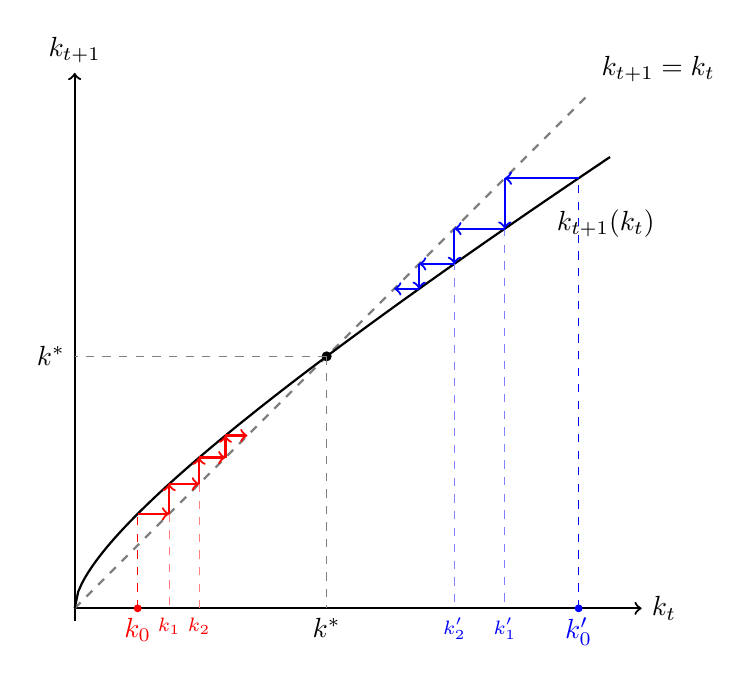
\begin{tikzpicture}[scale=0.8]
    % Axes
    \draw[->, thick] (0,-0.2) -- (0,8.5) node[above] {$k_{t+1}$};
    \draw[->, thick] (0,0) -- (9.0,0) node[right] {$k_t$};

    % 45-degree line
    \draw[thick, dashed, gray] (0,0) -- (8.2,8.2) node[above right, text=black] {$k_{t+1} = k_t$};

    % Transition Curve: y = 0.5x + sqrt(x)
    % Intersects 45-degree line exactly at k* = 4
    \draw[thick, black, domain=0:8.5, samples=150] plot (\x, {0.5*\x + sqrt(\x)});
    \node[black, below right] at (7.5, {0.5*7.5 + sqrt(7.5)}) {$k_{t+1}(k_t)$};

    % Steady State (4,4)
    \filldraw[black] (4,4) circle (2pt);
    \draw[dashed, gray] (4,4) -- (4,0) node[below, text=black] {$k^*$};
    \draw[dashed, gray] (4,4) -- (0,4) node[left, text=black] {$k^*$};

    % ==========================================
    % Path 1: Convergence from BELOW (Red)
    % Initial k_0 = 1
    % ==========================================
    \draw[dashed, red] (1,0) node[below] {$k_0$} -- (1,1.5);
    \filldraw[red] (1,0) circle (1.5pt);
    
    % Iteration 1
    \draw[->, red, thick] (1,1.5) -- (1.5,1.5);
    \draw[dashed, red!50] (1.5,1.5) -- (1.5,0) node[below, text=red] {\scriptsize $k_1$};
    % Iteration 2
    \draw[->, red, thick] (1.5,1.5) -- (1.5,1.975);
    \draw[->, red, thick] (1.5,1.975) -- (1.975,1.975);
    \draw[dashed, red!50] (1.975,1.975) -- (1.975,0) node[below, text=red] {\scriptsize $k_2$};
    % Iteration 3
    \draw[->, red, thick] (1.975,1.975) -- (1.975,2.393);
    \draw[->, red, thick] (1.975,2.393) -- (2.393,2.393);
    % Iteration 4
    \draw[->, red, thick] (2.393,2.393) -- (2.393,2.743);
    \draw[->, red, thick] (2.393,2.743) -- (2.743,2.743);

    % ==========================================
    % Path 2: Convergence from ABOVE (Blue)
    % Initial k'_0 = 8
    % ==========================================
    \draw[dashed, blue] (8,0) node[below] {$k'_0$} -- (8,6.828);
    \filldraw[blue] (8,0) circle (1.5pt);
    
    % Iteration 1
    \draw[->, blue, thick] (8,6.828) -- (6.828,6.828);
    \draw[dashed, blue!50] (6.828,6.828) -- (6.828,0) node[below, text=blue] {\scriptsize $k'_1$};
    % Iteration 2
    \draw[->, blue, thick] (6.828,6.828) -- (6.828,6.027);
    \draw[->, blue, thick] (6.828,6.027) -- (6.027,6.027);
    \draw[dashed, blue!50] (6.027,6.027) -- (6.027,0) node[below, text=blue] {\scriptsize $k'_2$};
    % Iteration 3
    \draw[->, blue, thick] (6.027,6.027) -- (6.027,5.468);
    \draw[->, blue, thick] (6.027,5.468) -- (5.468,5.468);
    % Iteration 4
    \draw[->, blue, thick] (5.468,5.468) -- (5.468,5.072);
    \draw[->, blue, thick] (5.468,5.072) -- (5.072,5.072);

\end{tikzpicture}
\end{center}

Based on the phase diagram and the mechanics of capital accumulation, we can derive two fundamental implications of the baseline Solow model:

\begin{itemize}
    \item \textbf{No Long-Run Growth:} In the absence of continuous technological progress, the economy inevitably converges to a fixed steady state ($k^*$). Once there, the growth rate of capital and output per worker strictly drops to zero. This implies that capital accumulation alone cannot act as the engine of sustained long-run economic growth.
    \item \textbf{Catch-Up Growth (Transitional Dynamics):} Economies starting further below their steady state will grow at a faster rate. The underlying mechanism is strictly driven by the \textit{diminishing marginal returns to capital}. When capital is scarce, its marginal product is exceptionally high, meaning investment vastly outpaces depreciation. As capital accumulates, the marginal returns diminish, causing the growth rate to gradually decelerate until the economy lands softly at the steady state.
\end{itemize}

\section{When Variables Change}

\subsection{Techonology Progress}

Suppose the economy has already reached its initial steady state $k^*$ with a technology level $A$. At a specific time $T$, technology unexpectedly and permanently improves to $A' > A$. 

Because capital per worker $k_t$ is a \textit{state variable} (evolution is durable), it cannot jump instantly at time $T$. However, the technological progress causes the economy's transition curve $k_{t+1}(k_t) = (1-\delta)k_t + sAf(k_t)$ to shift up vertically. Consequently, starting from time $T$, the economy begins to grow rapidly. Due to the pronounced diminishing returns, this ``catch-up growth" slows down quickly, and the capital stock $k_t$ transitions smoothly yet sharply towards the new, higher steady state $k^{*\prime}$.

\begin{center}
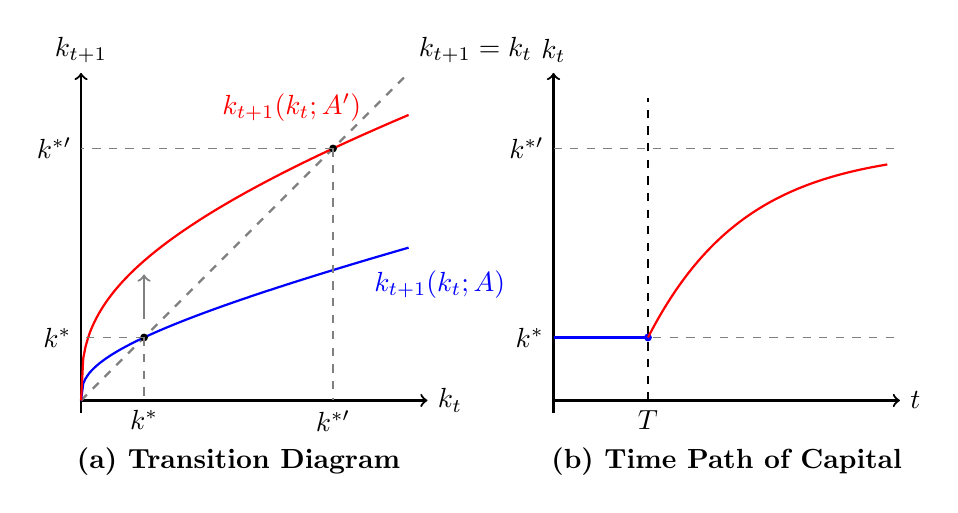
\begin{tikzpicture}[scale=0.8]
    % ==========================================
    % Left Panel: k_{t+1} vs k_t (Phase Diagram)
    % ==========================================
    \begin{scope}
        % Axes
        \draw[->, thick] (0,-0.2) -- (0,5.2) node[above] {$k_{t+1}$};
        \draw[->, thick] (0,0) -- (5.5,0) node[right] {$k_t$};
        
        % 45-degree line
        \draw[thick, dashed, gray] (0,0) -- (5.2,5.2) node[above right, text=black] {$k_{t+1} = k_t$};
        
        % Old Curve
        \draw[thick, blue, domain=0:5.2, samples=150] plot (\x, {0.2*\x + 0.8*pow(\x, 1/3)});
        \node[blue, below right] at (4.5, {0.2*4.5 + 0.8*pow(4.5, 1/3)}) {$k_{t+1}(k_t; A)$};
            
        % New Curve
        \draw[thick, red, domain=0:5.2, samples=150] plot (\x, {0.2*\x + 2.016*pow(\x, 1/3)});
        \node[red, above left] at (4.6, {0.2*4.6 + 2.016*pow(4.6, 1/3)}) {$k_{t+1}(k_t; A')$};
            
        % Mark old steady state
        \filldraw[black] (1,1) circle (1.5pt);
        \draw[dashed, gray] (1,1) -- (1,0) node[below, text=black] {$k^*$};
        \draw[dashed, gray] (1,1) -- (0,1) node[left, text=black] {$k^*$};
        
        % Mark new steady state
        \filldraw[black] (4,4) circle (1.5pt);
        \draw[dashed, gray] (4,4) -- (4,0) node[below, text=black] {$k^{*\prime}$};
        \draw[dashed, gray] (4,4) -- (0,4) node[left, text=black] {$k^{*\prime}$};
        
        % Point arrows indicating vertical shift at old k*
        \draw[->, thick, gray] (1.0, 1.3) -- (1.0, 2.0);
        
        % Label for panel
        \node[below] at (2.5,-0.6) {\textbf{(a) Transition Diagram}};
    \end{scope}

    % ==========================================
    % Right Panel: k_t vs t (Time Path)
    % ==========================================
    \begin{scope}[xshift=7.5cm]
        % Axes
        \draw[->, thick] (0,0) -- (5.5,0) node[right] {$t$};
        \draw[->, thick] (0,-0.2) -- (0,5.2) node[above] {$k_t$};
        
        % Mark Time T
        \draw[dashed] (1.5,0) node[below] {$T$} -- (1.5,4.8);
        
        % Steady state levels
        \draw[dashed, gray] (0,1) node[left, text=black] {$k^*$} -- (5.5,1);
        \draw[dashed, gray] (0,4) node[left, text=black] {$k^{*\prime}$} -- (5.5,4);
        
        % Path before T
        \draw[thick, blue] (0,1) -- (1.5,1);
        \filldraw[blue] (1.5,1) circle (1.5pt);
        
        % Path after T
        \draw[thick, red, domain=1.5:5.3, samples=150] plot (\x, {4 - 3*exp(-0.65*(\x-1.5))});
        
        % Label for panel
        \node[below] at (2.75,-0.6) {\textbf{(b) Time Path of Capital}};
    \end{scope}
\end{tikzpicture}
\end{center}

\subsection{One-Time Population Shock}

Suppose the economy has already reached its steady state $k^*$ with a given technology level $A$ and a constant population $L$. At a specific time $T$, the population exogenously and instantly increases to $L' > L$ (e.g., due to a sudden migration event).

Unlike a change in technology or saving rates, a one-time change in the level of population does not shift the transition curve $k_{t+1}(k_t)$. However, it directly impacts the per-worker state variable. Because the total capital stock $K_T$ is durable and fixed at time $T$, the sudden increase in the denominator $L$ causes the capital per worker $k_T$ to jump down instantly to a lower level, $k_T^{\prime} = K_T / L' < k^*$.

At this lower capital level, investment per worker now exceeds depreciation per worker. Consequently, starting from time $T$, the economy experiences temporarily high ``catch-up growth," accumulating capital per worker until it eventually converges back to the original steady state $k^*$. Take a special note that the total output $Y$ will be higher in the new steady state (due to more $L$), but output per worker $y^*$ remains unchanged.

\begin{center}
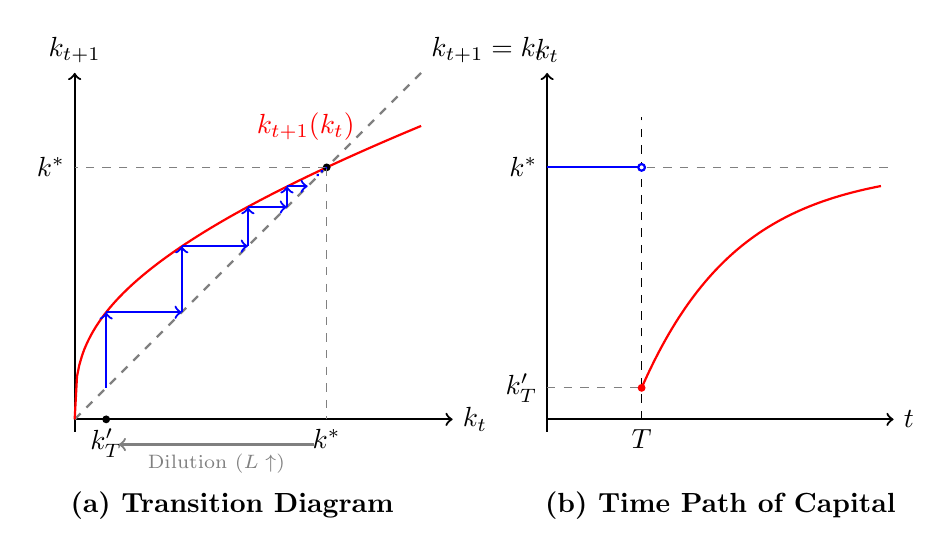
\begin{tikzpicture}[scale=0.8]
    % ==========================================
    % Left Panel: k_{t+1} vs k_t (Phase Diagram)
    % Showing FULL convergence path ALONG the curve.
    % ==========================================
    \begin{scope}
        % Axes
        \draw[->, thick] (0,-0.2) -- (0,5.5) node[above] {$k_{t+1}$};
        \draw[->, thick] (0,0) -- (6.0,0) node[right] {$k_t$};
        
        % 45-degree line
        \draw[thick, dashed, gray] (0,0) -- (5.5,5.5) node[above right, text=black] {$k_{t+1} = k_t$};
        
        % Transition Curve (No shift). delta=0.8, alpha=1/3, sA=2.016. SS k*=4.
        \draw[thick, red, domain=0:5.5, samples=150] plot (\x, {0.2*\x + 2.016*pow(\x, 1/3)});
        \node[red, above left] at (4.6, {0.2*4.6 + 2.016*pow(4.6, 1/3)}) {$k_{t+1}(k_t)$};
            
        % Mark Steady State k*
        \filldraw[black] (4,4) circle (1.5pt);
        \draw[dashed, gray] (4,4) -- (4,0) node[below, text=black] {$k^*$};
        \draw[dashed, gray] (4,4) -- (0,4) node[left, text=black] {$k^*$};
        
        % Mark diluted capital k'_T (Chosen at 0.5 to show multiple steps)
        \filldraw[black] (0.5,0) circle (1.5pt) node[below] {$k_T^{\prime}$};

        % Gray horizontal arrow indicating 'dilution' jump along x-axis from 4 to 0.5
        \draw[->, thick, gray] (3.8, -0.4) -- (0.7, -0.4);
        \node[gray, font=\scriptsize, anchor=north] at (2.25, -0.4) {Dilution ($L \uparrow$)};

        % --- FULL Convergence Cobbweb Path (Starting from x=0.5, SS=4) ---
        % Using precisely calculated coordinates for standard Solow params
        % delta=0.8, alpha=1/3, sA=2.016, k*=4, k_T'=0.5
        % Path color blue for contrast
        \draw[->, blue, thick] (0.5,0.5) -- (0.5, 1.70); % Vertical up to curve
        \draw[->, blue, thick] (0.5, 1.70) -- (1.70, 1.70); % Horizontal to 45deg

        \draw[->, blue, thick] (1.70, 1.70) -- (1.70, 2.75); % Vertical up to curve
        \draw[->, blue, thick] (1.70, 2.75) -- (2.75, 2.75); % Horizontal to 45deg

        \draw[->, blue, thick] (2.75, 2.75) -- (2.75, 3.37); % Vertical up to curve
        \draw[->, blue, thick] (2.75, 3.37) -- (3.37, 3.37); % Horizontal to 45deg

        \draw[->, blue, thick] (3.37, 3.37) -- (3.37, 3.70); % Vertical up to curve
        \draw[->, blue, thick] (3.37, 3.70) -- (3.70, 3.70); % Horizontal to 45deg
        
        % Add dotted lines to show continued convergence to SS
        \draw[dotted, blue, thick] (3.86, 3.86) -- (3.86, 3.94) -- (3.94, 3.94) -- (3.94, 3.97) -- (3.97, 3.97) -- (4,4);
        
        % Label for panel
        \node[below] at (2.5,-1.0) {\textbf{(a) Transition Diagram}};
    \end{scope}

    % ==========================================
    % Right Panel: k_t vs t (Time Path)
    % Noticeable fast convergence back up
    % ==========================================
    \begin{scope}[xshift=7.5cm]
        % Axes
        \draw[->, thick] (0,0) -- (5.5,0) node[right] {$t$};
        \draw[->, thick] (0,-0.2) -- (0,5.5) node[above] {$k_t$};
        
        % Mark Time T
        \draw[dashed] (1.5,0) node[below] {$T$} -- (1.5,4.8);
        
        % Steady state level (Returns to original)
        \draw[dashed, gray] (0,4) node[left, text=black] {$k^*$} -- (5.5,4);
        
        % Mark diluted level k'_T on y-axis (Matches phase diagram chosen level 0.5)
        \draw[dashed, gray] (0,0.5) node[left, text=black] {$k_T^{\prime}$} -- (1.5,0.5);
        
        % Path before T (Stationary at original k*)
        \draw[thick, blue] (0,4) -- (1.5,4);
        \filldraw[blue] (1.5,4) circle (1.5pt);
        
        % The Shock: Discontinuous jump down at T
        % Using fast convergence rate exp(-0.65*(t-T)) for sharpness
        \draw[thick, blue, fill=white] (1.5,4) circle (1.5pt); % Open circle at top
        \filldraw[red] (1.5,0.5) circle (1.5pt); % Closed circle at bottom
        
        % Path after T (Smooth, Concave catch-up growth back to original k*)
        % Adjust formula to match k'_T = 0.5 and k*=4: 4 - 3.5*exp(-0.65*(t-1.5))
        \draw[thick, red, domain=1.5:5.3, samples=150] plot (\x, {4 - 3.5*exp(-0.65*(\x-1.5))});
        
        % Label for panel
        \node[below] at (2.75,-1.0) {\textbf{(b) Time Path of Capital}};
    \end{scope}
\end{tikzpicture}
\end{center}

\section{Non-Autonomous Dynamics and the Balanced Growth Path}

What happens if technology grows exponentially over time, such that $A_t = A_0 e^{g_A \cdot t}$?

Now that the exogenous sequence $\{A_t\}_{t = 0}^{\infty}$ is known and strictly increasing, the Solow model becomes a \textit{non-autonomous} dynamic system.\footnote{
    In the theory of dynamical systems, a system is called \textit{autonomous} if its law of motion does not explicitly depend on time (i.e., $x_{t+1} = f(x_t)$). The baseline Solow model without technological progress is autonomous, yielding a single, fixed transition curve. When $A_t$ grows over time, the transition equation becomes $k_{t+1} = f(k_t, t)$. This explicit dependence on $t$ makes the system \textit{non-autonomous}, which graphically manifests as the transition curve shifting in every period.
} We can track the sequence of capital $\{k_t\}_{t = 0}^{\infty}$ by iterating the law of motion for $k_{t+1}$:
$$
\begin{aligned}
    k_1 & = (1-\delta)k_0 + s A_0 k_0^{\alpha} \\
    k_2 & = (1-\delta)k_1 + s A_1 k_1^{\alpha} \\
    k_3 & = (1-\delta)k_2 + s A_2 k_2^{\alpha} \\
    & \vdots
\end{aligned}
$$
Geometrically, instead of a single curve, we plot a \textit{family of curves} on the $(k_t, k_{t+1})$ phase plane:
$$
k_{t+1} = (1-\delta)k_t + s A_t k_t^{\alpha}
$$
Because $A_t$ is strictly increasing with $t$, the transition curve shifts upward every period.

% ------------------------------------------------------------------
% 将你刚刚画的 TikZ 代码放在这里 (保持原样即可)
% ------------------------------------------------------------------
\begin{center}
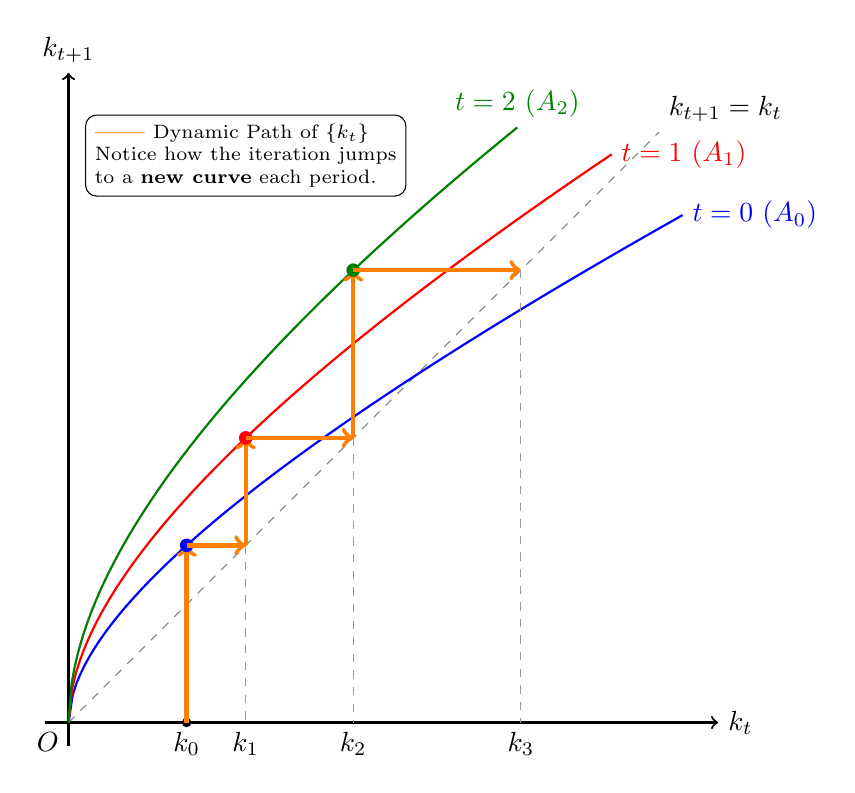
\begin{tikzpicture}[scale=1.5]
    % 坐标轴设置
    \draw[->, thick] (-0.2,0) -- (5.5,0) node[right] {$k_t$};
    \draw[->, thick] (0,-0.2) -- (0,5.5) node[above] {$k_{t+1}$};
    \node[below left] at (0,0) {$O$};

    % 绘制 45 度参考线 (k_{t+1} = k_t)
    \draw[dashed, gray] (0,0) -- (5.0,5.0) node[above right, black] {$k_{t+1}=k_t$};

    % 绘制一簇极度 Concave 的曲线
    \draw[blue, thick, domain=0:5.2, samples=150] plot (\x, {0.3*\x + 1.2*sqrt(\x)});
    \node[blue, right] at (5.2, {0.3*5.2 + 1.2*sqrt(5.2)}) {$t=0$ ($A_0$)};

    \draw[red, thick, domain=0:4.6, samples=150] plot (\x, {0.3*\x + 1.6*sqrt(\x)});
    \node[red, right] at (4.6, {0.3*4.6 + 1.6*sqrt(4.6)}) {$t=1$ ($A_1$)};

    \draw[green!50!black, thick, domain=0:3.8, samples=150] plot (\x, {0.3*\x + 2.0*sqrt(\x)});
    \node[green!50!black, above] at (3.8, {0.3*3.8 + 2.0*sqrt(3.8)}) {$t=2$ ($A_2$)};

    % 绘制动态迭代路径 (跨曲线跳跃)
    \draw[dashed, gray!80] (1.0, 0) node[below, text=black] {$k_0$} -- (1.0, 1.5);
    \filldraw[black] (1.0, 0) circle (1pt);

    \draw[->, ultra thick, orange] (1.0, 0) -- (1.0, 1.5);
    \filldraw[blue] (1.0, 1.5) circle (1.5pt); 
    \draw[->, ultra thick, orange] (1.0, 1.5) -- (1.5, 1.5);
    \draw[dashed, gray!80] (1.5, 1.5) -- (1.5, 0) node[below, text=black] {$k_1$};
    
    \draw[->, ultra thick, orange] (1.5, 1.5) -- (1.5, 2.41);
    \filldraw[red] (1.5, 2.41) circle (1.5pt); 
    \draw[->, ultra thick, orange] (1.5, 2.41) -- (2.41, 2.41);
    \draw[dashed, gray!80] (2.41, 2.41) -- (2.41, 0) node[below, text=black] {$k_2$};

    \draw[->, ultra thick, orange] (2.41, 2.41) -- (2.41, 3.83);
    \filldraw[green!50!black] (2.41, 3.83) circle (1.5pt); 
    \draw[->, ultra thick, orange] (2.41, 3.83) -- (3.83, 3.83);
    \draw[dashed, gray!80] (3.83, 3.83) -- (3.83, 0) node[below, text=black] {$k_3$};
    
    \node[draw, align=left, font=\scriptsize, fill=white, rounded corners] at (1.5, 4.8) {
        \textcolor{orange}{\textbf{\textemdash\textemdash}} Dynamic Path of $\{k_t\}$\\
        Notice how the iteration jumps\\
        to a \textbf{new curve} each period.
    };
\end{tikzpicture}
\end{center}

Since the transition curve is continuously shifting upward, a static steady state (where $k_{t+1} = k_t$) no longer exists. Instead, we look for a \textit{Balanced Growth Path}: a trajectory where key macroeconomic variables (like $k_t$ and $y_t$) grow at constant, time-invariant rates from the very first period.

\clmp{Existence of the Balanced Growth Path}{
    Given a constant growth rate of technology $g_A$, there exists a specific initial capital stock $k_0^*$ and a constant growth rate of capital $g_k$, such that the sequence:
    $$
    k_t = k_0^* e^{g_k \cdot t}
    $$
    is an exact solution to the dynamic model for all $t \ge 0$.
}{
    We construct the proof using the standard \textit{Guess and Verify} method.
    \begin{itemize}
        \item \textbf{Step 1: Guess}\\
    Suppose the claim is true, meaning $k_t$ grows at a constant rate $g_k$. We substitute $k_t = k_0 e^{g_k t}$ and $k_{t+1} = k_0 e^{g_k (t+1)}$ into the law of motion:
    $$
    k_0 e^{g_k(t+1)} = (1-\delta) k_0 e^{g_k t} + s A_0 e^{g_A t} \left(k_0 e^{g_k t}\right)^{\alpha}
    $$
    \item \textbf{Step 2: Verify by matching coefficients}\\
    Divide both sides by the term $k_0 e^{g_k t}$:
    $$
    e^{g_k} = (1-\delta) + s A_0 k_0^{\alpha-1} e^{g_A t} e^{\alpha g_k t} e^{-g_k t}
    $$
    Rearranging the terms yields:
    $$
    e^{g_k} + \delta - 1 = s A_0 k_0^{\alpha-1} e^{\left[g_A + (\alpha-1)g_k\right] t}
    $$
    For this equation to hold true for \textit{all} $t$ (which is the definition of balanced growth), the right-hand side must be independent of time $t$. Therefore, the exponent on $e$ must be exactly zero:
    $$
    g_A + (\alpha-1)g_k = 0 \implies g_k = \frac{g_A}{1-\alpha}
    $$
    \item \textbf{Step 3: Pin down the initial condition $k_0^*$}\\
    Now that the exponential term is $e^0 = 1$, we can solve for the unique initial capital $k_0^*$ that places the economy immediately on the BGP:
    $$
    k_0^* = \left( \frac{s A_0}{e^{g_k} + \delta - 1} \right)^{\frac{1}{1-\alpha}}
    $$
    As long as the economy starts at this specific $k_0^*$, capital will grow forever at the constant rate $g_k = g_A / (1-\alpha)$.
    \end{itemize}
}

\section{The Lucas Critique}

\state{Lucas Critique}{
    Assuming structural parameters remain invariant to policy or environmental changes leads to systematic forecasting errors.
}

One of the most fundamental criticisms of the baseline Solow model is its assumption that the saving rate $s$ is an exogenous constant. In reality, saving is an optimal choice made by forward-looking households. If the economic environment changes, rational agents will adjust their behavior.

Consider a positive technological shock ($A \uparrow$). In the standard Solow model, the investment curve mechanically shifts up, determining a new ``naive" steady state. However, if the technological improvement alters the return to capital or lifetime income, the household's optimal saving rate $s$ will also change.
\begin{itemize}
    \item \textbf{Understating the Effect:} If an increase in $A$ incentivizes households to save more ($s \uparrow$), the investment curve shifts up twice: once due to $A$, and again due to $s$. The naive Solow model will \textit{understate} the true increase in steady-state capital.
    \item \textbf{Overstating the Effect:} Conversely, if higher $A$ leads to a wealth effect that causes households to consume more and save less ($s \downarrow$), the secondary downward shift in $s$ partially offsets the initial shock. The naive Solow model will \textit{overstate} the true impact.
\end{itemize}

\vspace{1em}
\begin{figure}[htbp]
    \centering
    % 左图: s 随 A 增加 (Understate)
    \begin{minipage}{0.48\textwidth}
        \centering
        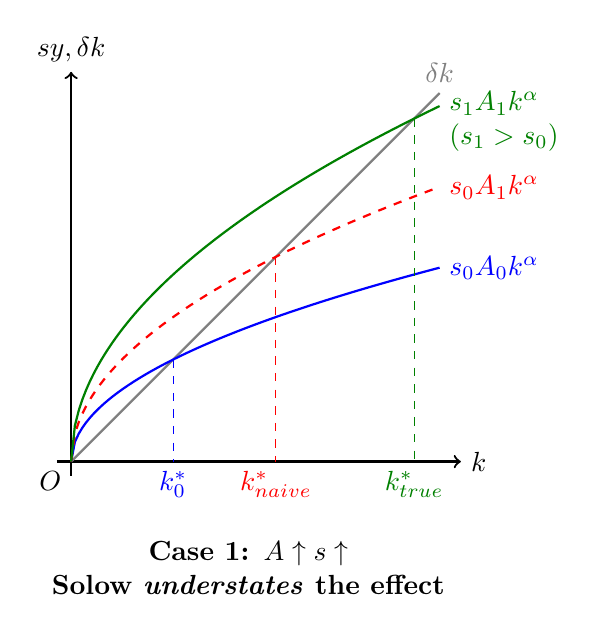
\begin{tikzpicture}[scale=0.9]
            % Axes
            \draw[->, thick] (-0.2,0) -- (5.5,0) node[right] {$k$};
            \draw[->, thick] (0,-0.2) -- (0,5.5) node[above] {$sy, \delta k$};
            \node[below left] at (0,0) {$O$};
            
            % Depreciation line (\delta k) - y = x
            % 改动：将 \delta k 放到线段末端的正上方
            \draw[thick, gray] (0,0) -- (5.2,5.2) node[above] {$\delta k$};
            
            % 1. Base Curve (c=1.2, x=1.44)
            \draw[blue, thick, domain=0:5.2, samples=100] plot (\x, {1.2*sqrt(\x)});
            \draw[dashed, blue] (1.44, 1.44) -- (1.44, 0) node[below] {$k_0^*$};
            \node[blue, right] at (5.2, 2.73) {$s_0 A_0 k^\alpha$};
            
            % 2. Naive Curve (only A increases, c=1.7, x=2.89)
            \draw[red, thick, dashed, domain=0:5.2, samples=100] plot (\x, {1.7*sqrt(\x)});
            \draw[dashed, red] (2.89, 2.89) -- (2.89, 0) node[below] {$k_{naive}^*$};
            \node[red, right] at (5.2, 3.87) {$s_0 A_1 k^\alpha$};
            
            % 3. True Curve (A increases AND s increases, c=2.2, x=4.84)
            \draw[green!50!black, thick, domain=0:5.2, samples=100] plot (\x, {2.2*sqrt(\x)});
            \draw[dashed, green!50!black] (4.84, 4.84) -- (4.84, 0) node[below] {$k_{true}^*$};
            % 改动：稍微下调绿色文本的 y 坐标，避开 \delta k
            \node[green!50!black, right, align=left] at (5.2, 4.8) {$s_1 A_1 k^\alpha$\\($s_1 > s_0$)};
            
            % Title
            % 改动：下调标题 y 坐标到 -1.5，避开横坐标的 k^* 标注
            \node[align=center, font=\bfseries] at (2.5, -1.5) {Case 1: $A \uparrow \implies s \uparrow$\\ Solow \textit{understates} the effect};
        \end{tikzpicture}
    \end{minipage}
    \hfill
    % 右图: s 随 A 减少 (Overstate)
    \begin{minipage}{0.48\textwidth}
        \centering
        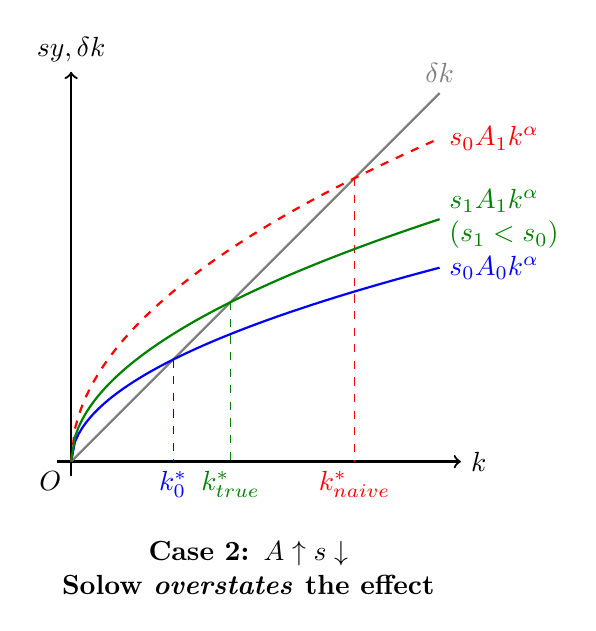
\begin{tikzpicture}[scale=0.9]
            % Axes
            \draw[->, thick] (-0.2,0) -- (5.5,0) node[right] {$k$};
            \draw[->, thick] (0,-0.2) -- (0,5.5) node[above] {$sy, \delta k$};
            \node[below left] at (0,0) {$O$};
            
            % Depreciation line (\delta k) - y = x
            \draw[thick, gray] (0,0) -- (5.2,5.2) node[above] {$\delta k$};
            
            % 1. Base Curve (c=1.2, x=1.44)
            \draw[blue, thick, domain=0:5.2, samples=100] plot (\x, {1.2*sqrt(\x)});
            \draw[dashed, blue] (1.44, 1.44) -- (1.44, 0) node[below] {$k_0^*$};
            \node[blue, right] at (5.2, 2.73) {$s_0 A_0 k^\alpha$};
            
            % 2. Naive Curve (only A increases, c=2.0, x=4.0)
            \draw[red, thick, dashed, domain=0:5.2, samples=100] plot (\x, {2.0*sqrt(\x)});
            \draw[dashed, red] (4.0, 4.0) -- (4.0, 0) node[below] {$k_{naive}^*$};
            \node[red, right] at (5.2, 4.56) {$s_0 A_1 k^\alpha$};
            
            % 3. True Curve (A increases BUT s decreases, c=1.5, x=2.25)
            \draw[green!50!black, thick, domain=0:5.2, samples=100] plot (\x, {1.5*sqrt(\x)});
            \draw[dashed, green!50!black] (2.25, 2.25) -- (2.25, 0) node[below] {$k_{true}^*$};
            \node[green!50!black, right, align=left] at (5.2, 3.42) {$s_1 A_1 k^\alpha$\\($s_1 < s_0$)};
            
            % Title
            % 改动：下调标题 y 坐标到 -1.5
            \node[align=center, font=\bfseries] at (2.5, -1.5) {Case 2: $A \uparrow \implies s \downarrow$\\ Solow \textit{overstates} the effect};
        \end{tikzpicture}
    \end{minipage}
\end{figure}


The true profundity of the Lucas Critique extends far beyond a simple complaint about the Solow model's saving rate. It sparked a methodological revolution that forced modern macroeconomics to develop rigorous \textit{micro-foundations}. 

Prior to Lucas (1976), macro-econometric models relied heavily on historical relationships between aggregate variables (treating variables like $s$ or the marginal propensity to consume as structural constants). Lucas argued that these are merely \textit{reduced-form} outcomes of underlying optimization problems. When the government changes an economic policy or when technology shifts, the constraints of the optimization problem change, and rational agents will immediately alter their behavior. Consequently, historical data becomes useless for predicting the effects of new policies.

To avoid the Lucas Critique, macroeconomic models must be built upon \textit{deep parameters} (or structural parameters) that are genuinely invariant to policy changes. These include:
\begin{itemize}
    \item \textbf{Preferences:} Time discount factor ($\beta$), coefficient of relative risk aversion ($\gamma$).
    \item \textbf{Technology:} Capital share ($\alpha$), depreciation rate ($\delta$).
\end{itemize}

This critique naturally paves the way for the next evolution in our theory: the \textit{Neoclassical Growth Model} (often formalized as the \textit{Ramsey-Cass-Koopmans model}). Instead of assuming an exogenous saving rule, this framework models the economy as a dynamic general equilibrium where households and firms actively optimize. In such a micro-founded setting, the saving behavior organically emerges as an endogenous outcome, perfectly immune to the Lucas Critique.

